% Chapter Template

\chapter{Results and Discussion} % Main chapter title

\label{Chapter4} % Change X to a consecutive number; for referencing this chapter elsewhere, use \ref{ChapterX}

\lhead{Chapter 4. \emph{Results and Discussion}} % Change X to a consecutive number; this is for the header on each page - perhaps a shortened title

%----------------------------------------------------------------------------------------
%	SECTION 1
%----------------------------------------------------------------------------------------

\section{Artificial Neural Network (ANN) Results}
The relationship between the microstructure and mechanical behaviour of DP steels is extremely complex. Successful implementation of an ANN model would have helped understand these complex relations and helped in predicting experimental behavior of other heterogeneous systems. For assessing our model's predictive capabilities over three different variables simultaneously, a metric is used to estimate how well the model performs for each of these variables. For this purpose, we calculate the coefficient of determination, $R^2$. $R^2$ represents the proportion of variance that has been explained by the independent variables in the model. It provides an indication of goodness of fit and therefore a measure of how well unseen samples are likely to be predicted by the model, through the proportion of explained variance. Best possible score is 1.0 and it can be negative (because the model can be arbitrarily worse). This metric is given by the following equation:
\begin{equation}
    R^2(y, \hat{y}) = 1 - \frac{\sum_{i=1}^{n} (y_i - \hat{y}_i)^2}{\sum_{i=1}^{n} (y_i - \bar{y})^2}
\end{equation}
where $y$ is the actual output (true value) and $\hat{y}$ is the prediction made by the ANN model. For a model with $100\%$ accuracy then $y_i = \hat{y}_i)$ for all $i's$ making $R^2 = 1$, which indeed is the best case scenario. 

A number of neural network architectures were trained and their $R^2$ and mean squared error values were recorded for a comparative parametric study. The following table shows the results that were obtained along with the time taken to train each model. 

\begin{table}
\begin{center}
\begin{tabular}{|c|c|c|c|c|c|c|}
\hline
Layers & Architecture & MSE & Time & \multicolumn{3}{c|}{$R^2$} \\
\hline
&(Neurons in every layer) & & (hrs)& ${\bar{\epsilon}}$ & $\bar{\sigma}$ & tri \\
\hline
2 & 8,4 & 0.0221 & 1.44 & 0.55 & 0.16 & 0.7 \\
3 & 16,8,4, & 0.0221 & 1.76 & 0.55 & 0.16 & 0.07 \\
4 & 32,16,8,4 & 0.0221 & 1.78 & 0.55 & 0.17 & 0.06 \\
5 & 64,32,16,8,4 & 0.0222 & 1.82 & 0.55 & 0.15 & 0.05 \\
6 & 128, 64,32,16,8,4 & 0.0266 & 1.87 & 0.16 & 0.13 & 0.02 \\
7 & 256,128,64,32,16,8,4 & 0.0290 & 3.47 & $<0$ & $<0$ & $<0$ \\
8 & 512,256,128,64,32,16,8,4 & 0.0290 & 4.59 & $<0$ & $<0$ & $<0$ \\
9 & 1024,512,256,128,64,32,16,8,4 & 0.0289 & 7.32 & $<0$ & $<0$ & $<0$ \\
11 & 1024,1024,512,512,256,128,64,32,16,8,4 & 0.0290 & 20.24 & $<0$ & $<0$ & $<0$ \\
\hline
\end{tabular}
\end{center}
\caption{\label{tab:diff-ann-table}Study of accuracy of models with different depths and neurons.}
\end{table}

As can be clearly seen from the table, the model is unable to make the predictions successfully. The MSE is very high and the $R^2$ values too low. For the model to be acceptable, the MSE values should have been in the range of $10^{-4} - 10^{-5}$ and $R^2$ values should be above $0.80$. All the above simulations have run for 5 epochs. Increasing the epochs is usually accompanied by a decrease in error. However, even after increasing to 20 epochs, the $R^2$ values did not improve. The first architecture in Table \ref{tab:diff-ann-table} was trained for 20 epochs. The MSE reduced to 0.0216, but $R^2$ values remained approximately the same. Increasing the epochs increased the training time to 8.5 hours without yielding any significant results.  Increasing the dept and complexity of the network is another way to increase the accuracy. However, as can be seen from the table, the MSE and $R^2$ values actually worsen as the number of hidden layers are increased beyond 4. Another major drawback in the ANN model is the limited dataset we are using to train it. The data consists of only discrete data at $0.01$ strain intervals. If instead, we trained our data to smaller strain intervals of the FE simulations, the results would be perhaps better, albeit at the cost of significant training times.

ANN predicted values are plotted in Figure \ref{fig:exp_pred_ann} against the ground truth values to better visualize the performance of our model. Note that all results are plotted on the normalized scales. For an ideal case, all the data points would lie as close to the $y=x$ line.
\begin{figure}[!h]
	\centering
	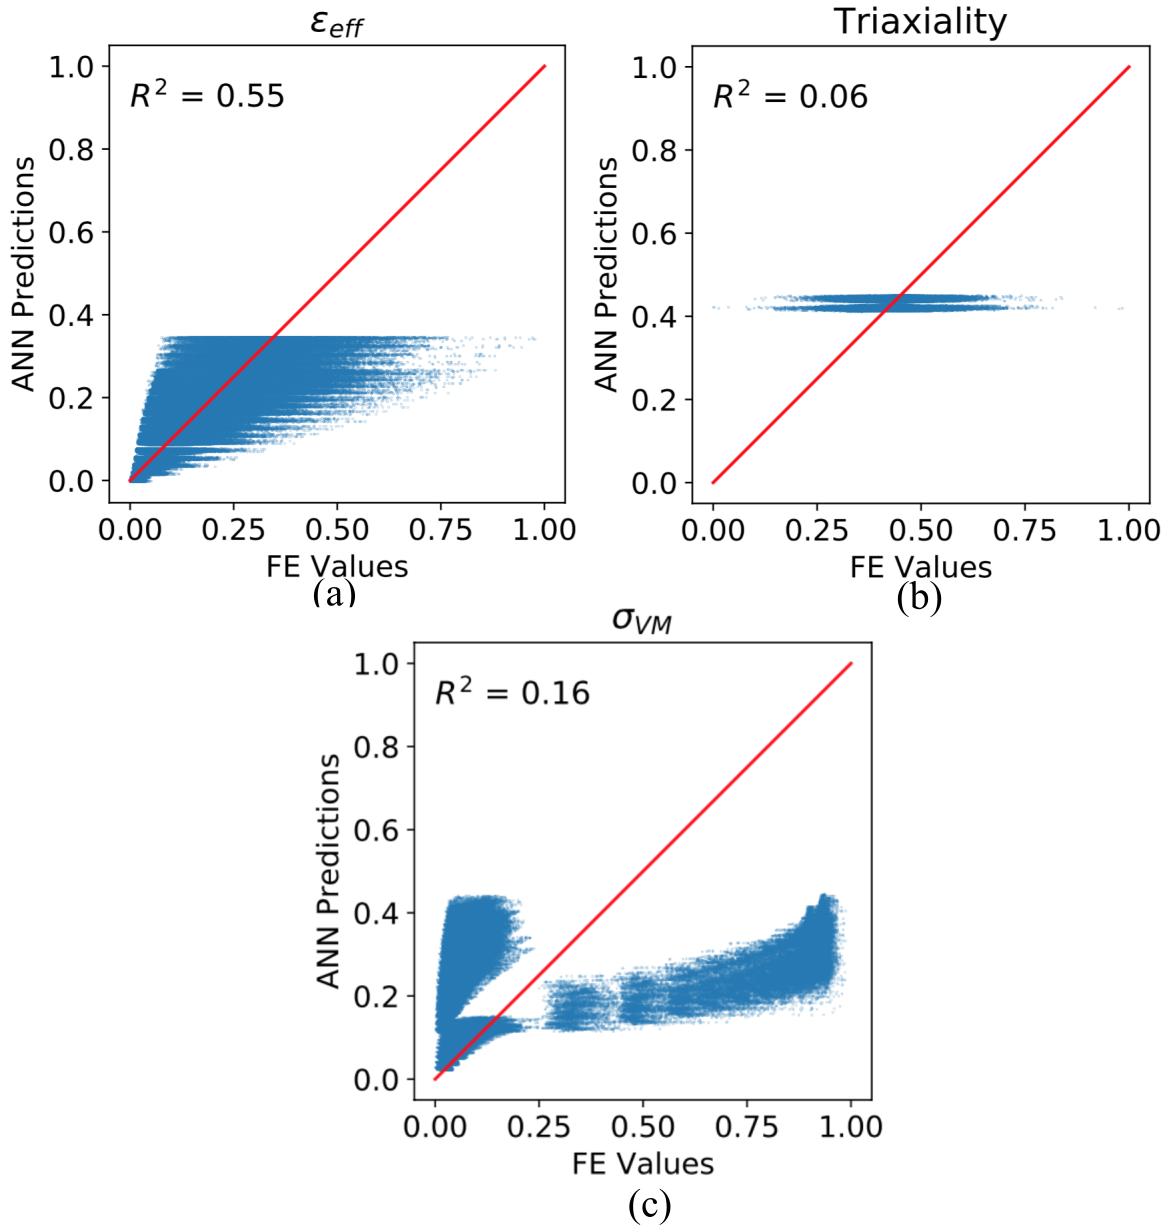
\includegraphics[width=0.9\textwidth]{Pictures/ann-res/final-ann-bitmap.png}
	\hspace{1mm}
	\caption{Plot of ANN predicted values vs FE values for (a) effective strain, (b) stress triaxiality ratio, and (c) von Mises effective stress. Note that all the variables are normalized.} 
	\label{fig:exp_pred_ann}
\end{figure}
A separate model was also trained to predict only one variable, effective strain. The architecture was kept the same, and the results showed an improvement in the $R^2$ value. We can conclude that predicting multiple variables using a single ANN leads to inaccuracy. Figure-\ref{fig:r2-ann} shows the $R^2$ values and figure-\ref{fig:ann-contours} shows the contour plots of ANN predicted value as compared to the true values. The numerical value of the predictions is quite inaccurate however, the ANN model has been able to locate some hotspots. 
\begin{figure}[!h]
	\centering
	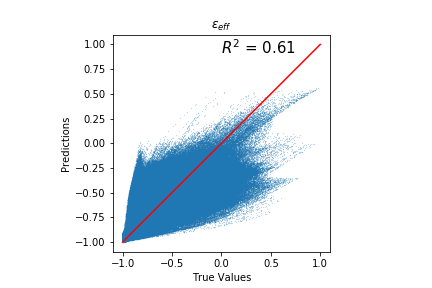
\includegraphics[width=0.9\textwidth]{Pictures/strain_eff_pred_exp.png}
	\hspace{1mm}
	\caption{Plot of ANN predicted values vs FE values for effective strain trained alone} 
	\label{fig:r2-ann}
\end{figure}

\begin{figure}[!h]
	\centering
	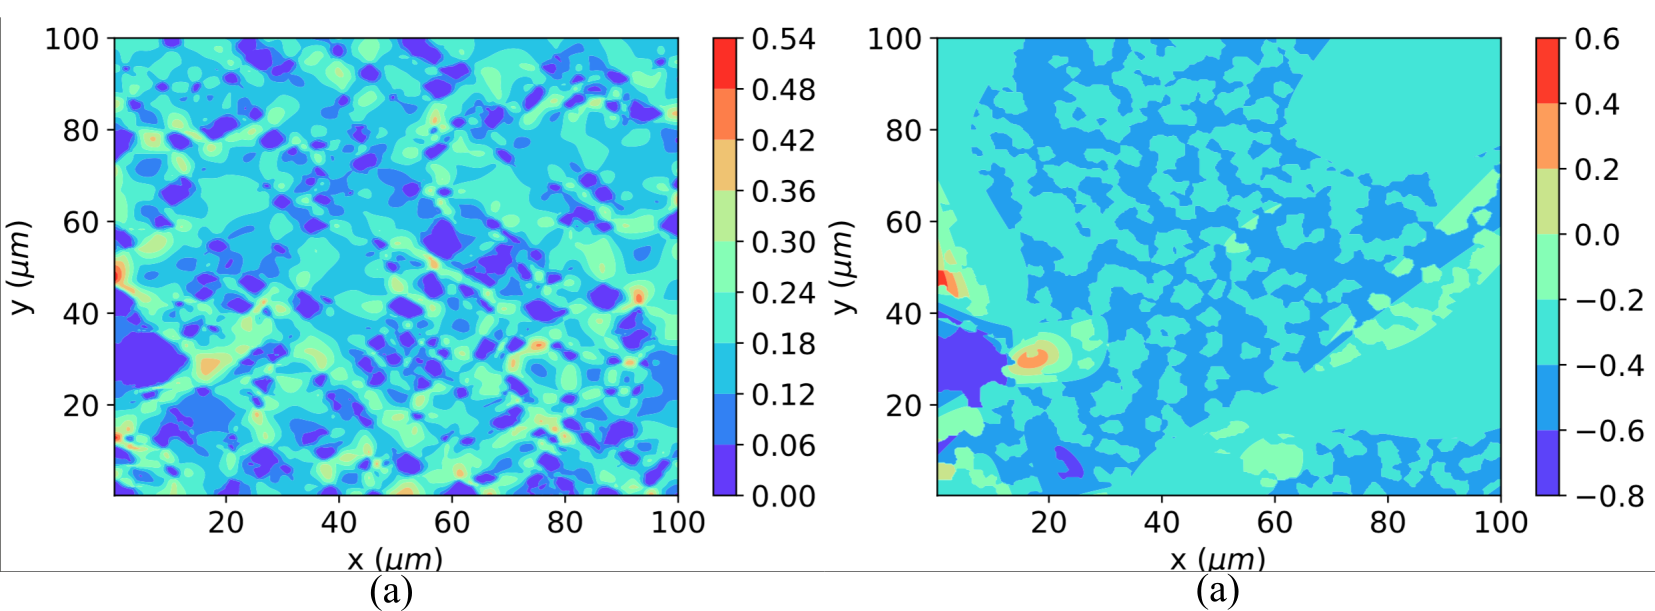
\includegraphics[width=0.95\textwidth]{Pictures/ann-res/ann-contours.png}
	\hspace{1mm}
	\caption{Effective Strain contour plots for (a) FE and (b) ANN predicted values.} 
	\label{fig:ann-contours}
\end{figure}
\newpage
\section{LSTM Model Results}
The LSTM Model shows significantly better performance than the ANN model. Plastic deformation being a history-dependent process, the output variable prediction is better modeled using LSTMs as they treat data as a time series. LSTMs maintain a context over time making them efficient in time series predictive modeling problems. Our model was able to achieve very high $R^2$ values for all the three output variables here, namely, effective strain (${\bar{\epsilon}}$), von Mises effective stress ($\bar{\sigma}$) and stress triaxiality ratio. The high accuracy of the model can be observed from the plots in
Figure \ref{fig:exp_pred_lstm}. Table \ref{tab:diff-lstm-table} shows results from LSTM models trained with different number of layers. Each layer contains 200 neurons and all the models take under 15 minutes to train. The training time here is 7 times less than our best ANN model. 

\begin{table}
\begin{center}
\begin{tabular}{|c|c|c|c|c|c|}
\hline
Layers & MSE & \multicolumn{3}{c|}{$R^2$} \\
\hline
 & & ${\bar{\epsilon}}$ & $\bar{\sigma}$ & tri \\
\hline
2 & $2.93 \times 10^{-6}$ & 0.89 & 0.99 & 0.51\\
4 & $2.78 \times 10^{-5}$ & 0.89 & 0.89 & 0.92\\
8 & $4.74 \times 10^{-5}$ & 0.90 & 0.96 & 0.97\\
16 & $0.02$ & -1.20 & 0.93 & 0.96\\
\hline
\end{tabular}
\end{center}
\caption{Study of accuracy of models with different depths. All layers have 200 neurons.}
\label{tab:diff-lstm-table}
\end{table}
\begin{figure}[!h]
	\centering
	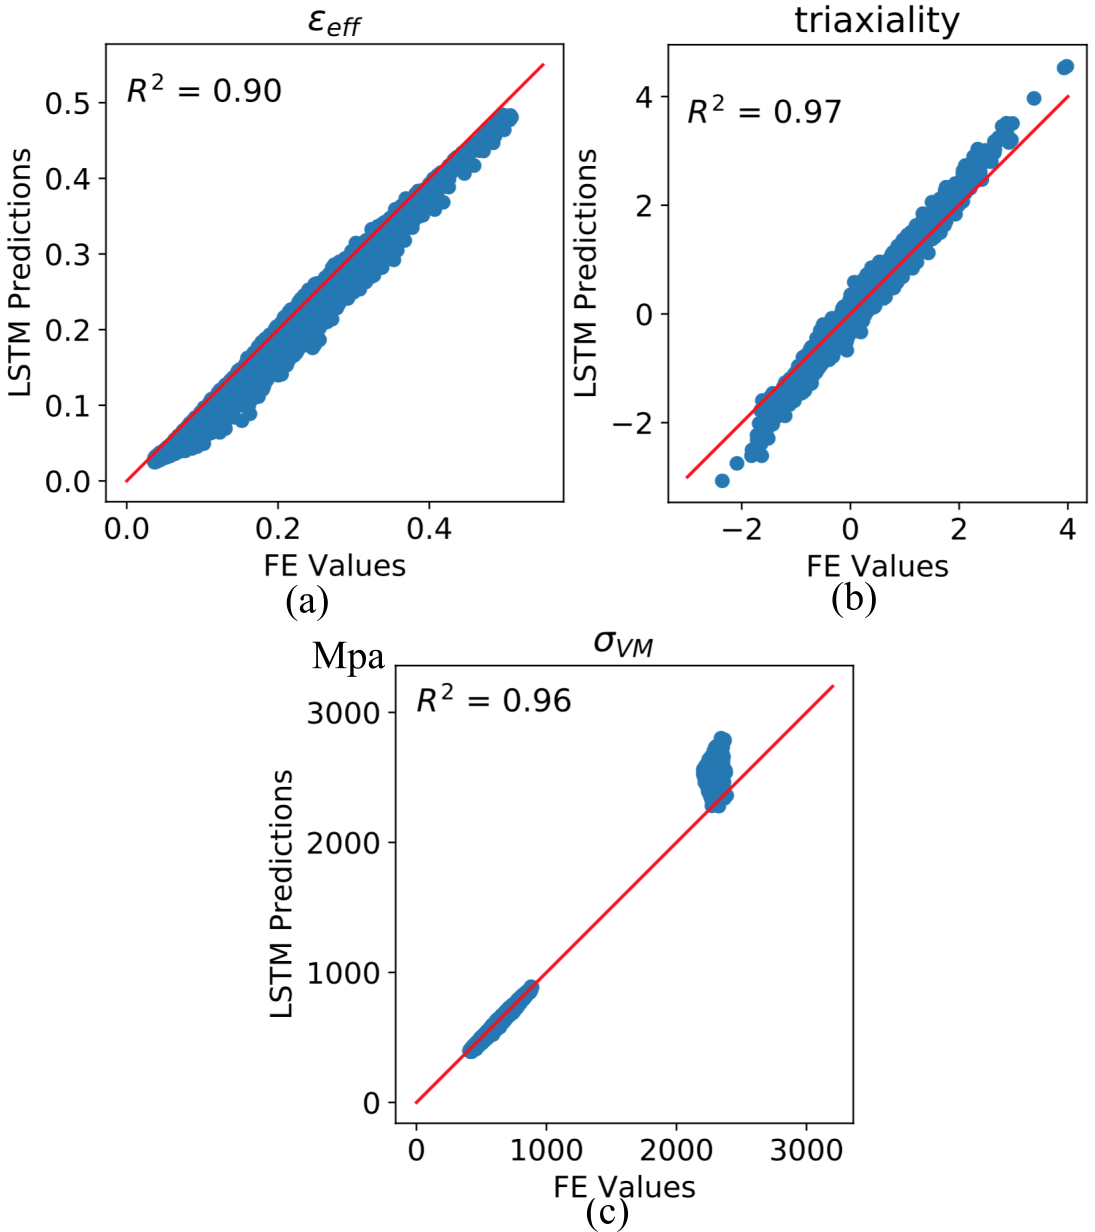
\includegraphics[width=0.8\textwidth]{Pictures/lstm-res/final-lstm-bitmap.png}
	\hspace{1mm}
	\caption{Plot of LSTM predicted values vs FE values for (a) effective strain, (b) triaxiality, (c) von Mises effective stress. Note that all the variables are normalized.} 
	\label{fig:exp_pred_lstm}
\end{figure}

Finally, figures \ref{fig:eff_strain_bitmap}, \ref{fig:tri_bitmap} and \ref{fig:vonmises_bitmap} show the contour plots for the different predicted variable at the last strain step. The contour plots depict how the model has successfully captured local behaviour of the microstructure. In figure-\ref{fig:vonmises_bitmap}, the predicted stress values higher than the FE values but the regions with high stress have been captured with good accuracy.
% \begin{figure}[hbtp]
% \begin{center}
% 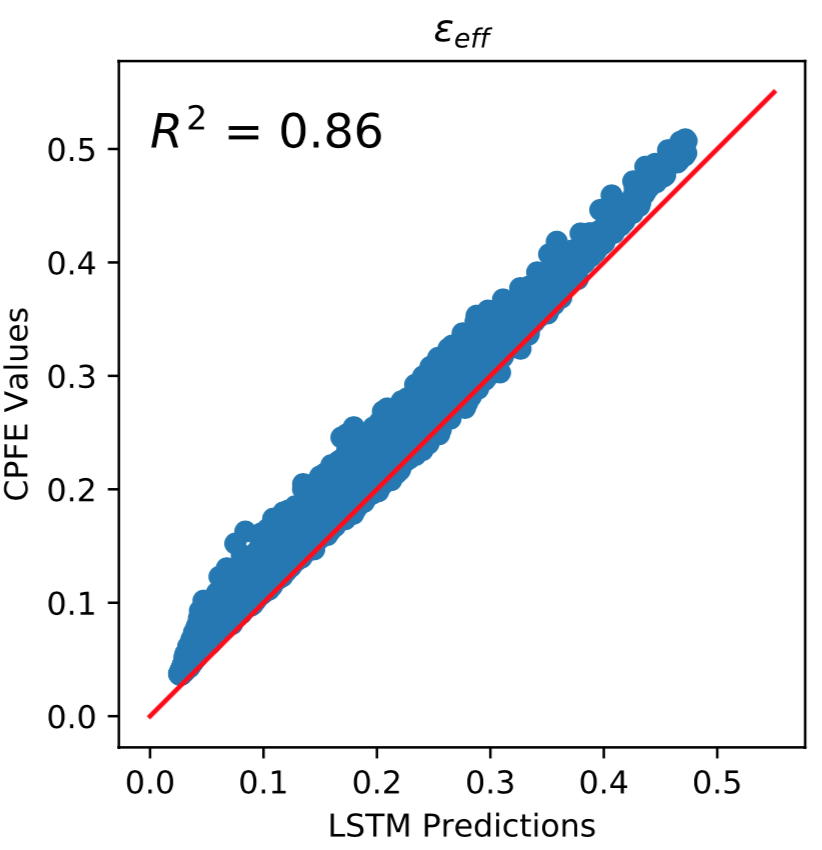
\includegraphics[scale=0.4]{Pictures/lstm-res/strain_eff.png}
% 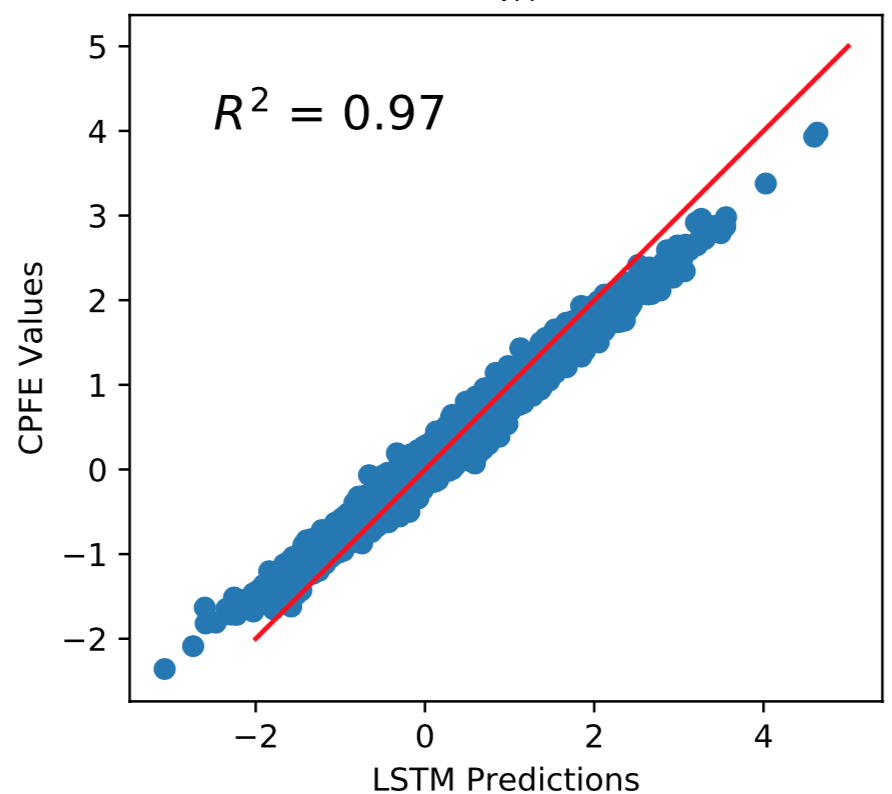
\includegraphics[scale=0.4]{Pictures/lstm-res/tri.png}
% \end{center}
% \begin{center}
% 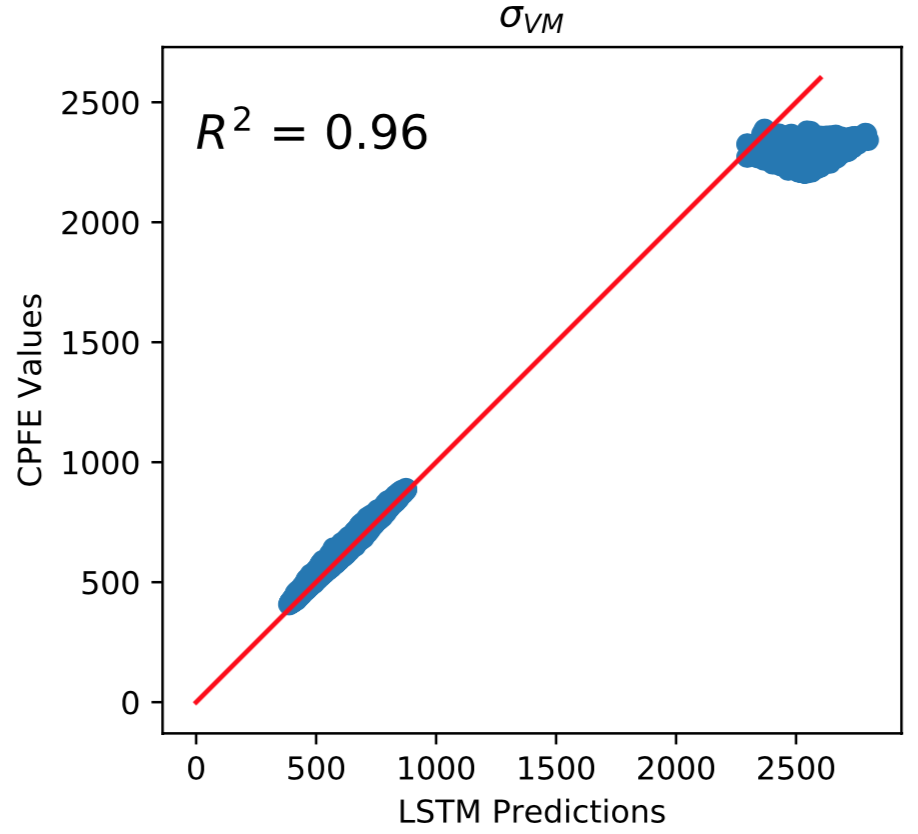
\includegraphics[scale=0.4]{Pictures/lstm-res/vonmises.png}
% \end{center}
% \caption{Plots of ANN Predictions vs CPFE Values for all the output variables}
% \label{fig:exp_pred_lstm}
% \end{figure}

\begin{figure}[!h]
	\centering
	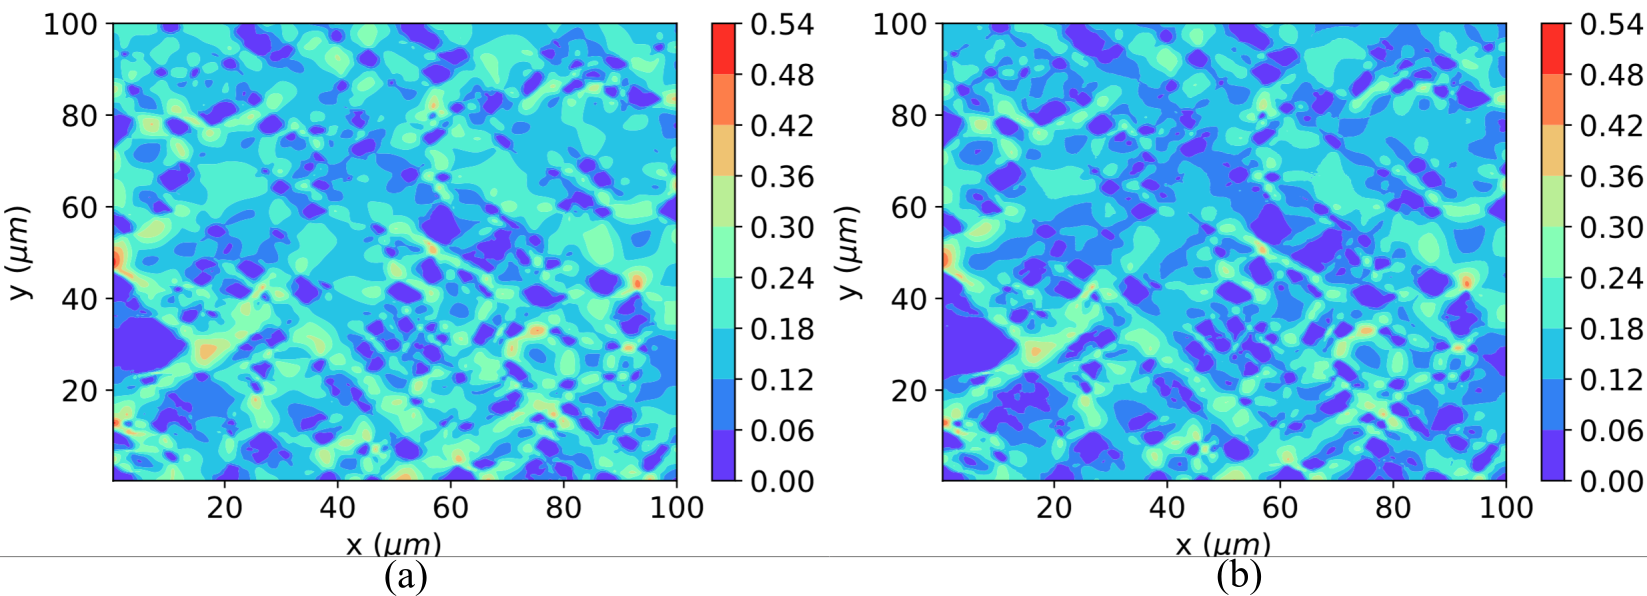
\includegraphics[width=0.95\textwidth]{Pictures/lstm-res/eff_strain_bitmap.png}
	\hspace{1mm}
	\caption{Effective Strain contour plots for (a) FE and (b) LSTM predicted values.} 
	\label{fig:eff_strain_bitmap}
\end{figure}

\begin{figure}[!h]
	\centering
	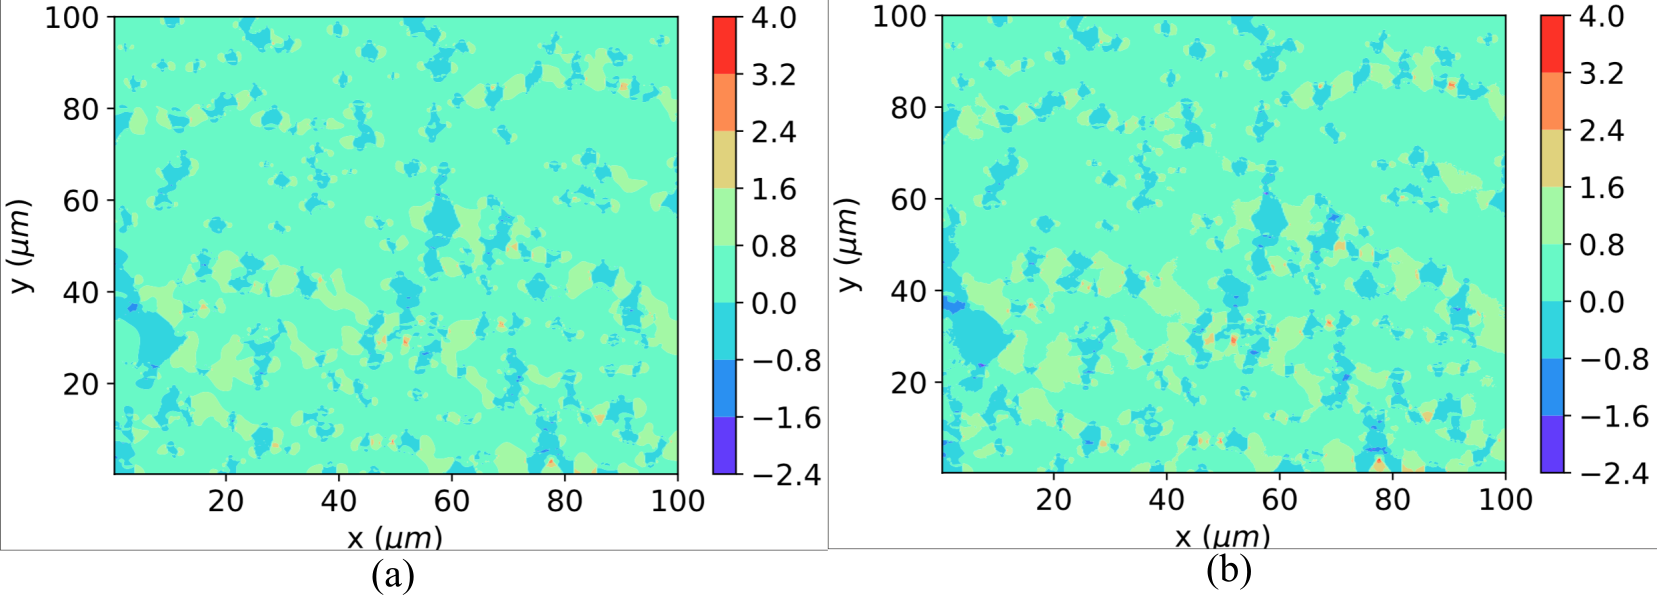
\includegraphics[width=0.95\textwidth]{Pictures/lstm-res/tri_bitmap.png}
	\hspace{1mm}
	\caption{Triaxiality contour plots for (a) FE and (b) LSTM predicted values.} 
	\label{fig:tri_bitmap}
\end{figure}

\begin{figure}[!h]
    \centering
	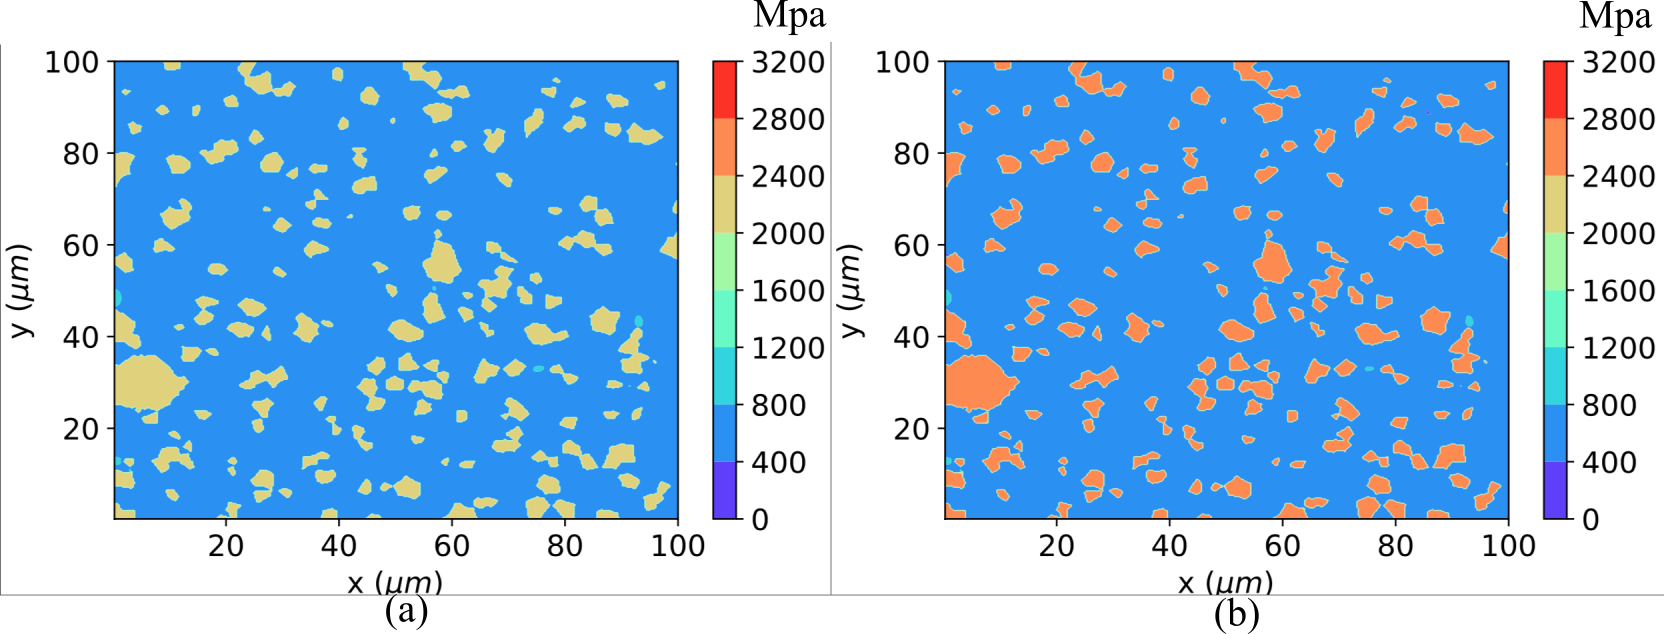
\includegraphics[width=0.95\textwidth]{Pictures/lstm-res/vonmises_bitmap-units.png}
	\hspace{1mm}
	\caption{Vonmises contour plots for (a) FE and (b) LSTM predicted values.} 
	\label{fig:vonmises_bitmap}
\end{figure}